\section{Основная часть}

В данном разделе рассмотреннно расширение языка YARD и модификация алгоритма синтаксического анализа GLL.


\subsection{Архитектура}

Ввиду модульной структуры проекта YaccConstructor, задействованную структуру проекта можно разделить на части, показанные на рисунке~\ref{project_structure}.

В проекте используется язык описания грамматик YARD~\cite{YARD}, который поддерживает различные конструкции, упрощающие разработку грамматик: повторения \verb|x*[1..10]|, дизъюнкции \texttt{A|B}, условное вхождние и подобные. Перед подачей генератору, дерево разбора грамматики проходит через множество преобразований, в результате которых, грамматика приводится к форме Бэкуса-Наура~\cite{BNF}.

\begin{figure}[h]
\centering
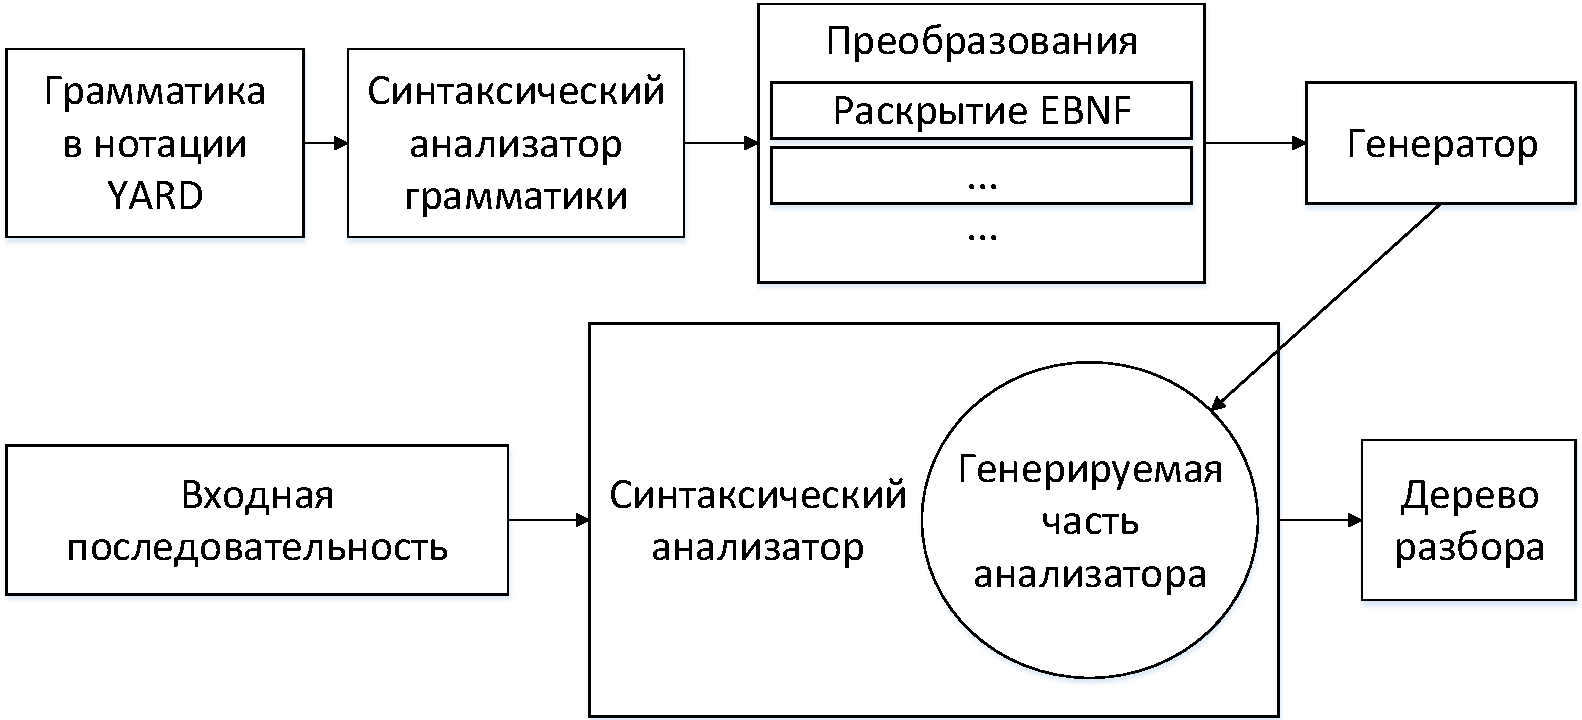
\includegraphics[width=\textwidth]{Gorokhov/courseworkpictures/img2.pdf}
\caption{Структура существующего решения}
\label{project_structure}
\end{figure}

\subsection{Расширение YARD}
Для работы с конъюнктивными грамматиками в язык YARD была добавлена новая конструкция: конъюнкция, приоритет которой между дизъюнкцией и последовательностью. Язык YARD поддерживает различные конструкции вроде повторений (x*[1..10]), которые преобразуются перед подачей генератору. Так как в язык была добавлена новая конструкция, нужно было обеспечить её поддержку во всех существующих преобразованиях.

Кроме того, добавленную конструкцию также необходимо преобразовывать к виду, принимаемому генератором. Предлагается следующее решение: грамматика преобразовывается к контекстно-свободной, с дополнительной информацией о существовании конъюнкции. Для каждой конъюнкции в грамматике создаётся три новых правила: по одному на каждый конъюнкт и одно на дизъюнкцию конъюнктов, в исходном правиле конъюнкция заменяется ссылкой на правило с дизъюнкцией конъюнктов. На рисунках~\ref{grammar0} и~\ref{grammar1} показан пример начальной грамматики ($G_{0}$) и результат её преобразования ($G_{1}$). В правиле \verb|S| содержится конъюнкция, которая заменяется на ссылку на сгенерированное правило \verb|Conj0|. Для каждого из конъюнктов также генерируется правило и продукция правила \verb|Conj0| представляет собой выбор между ними.

\begin{figure}
$$
\begin{array}{crcl}
& \mbox{\texttt{ S }} &::=& \mbox{\texttt{ A D }} \& \mbox{\texttt{ B}} \\
& \mbox{\texttt{ A }} & ::=& \mbox{\texttt{ A a |}}  \epsilon \\
& \mbox{\texttt{ D }} & ::=& \mbox{\texttt{ A d |}}  \epsilon \\
& \mbox{\texttt{ B }} & ::=& \mbox{\texttt{ A b D |}}\epsilon \\
\end{array}
$$
\caption{Грамматика $G_{0}$}
\label{grammar0}
\end{figure}


\begin{figure}
$$
\begin{array}{crcl}
& \mbox{\texttt{ S }} &::=& \mbox{\texttt{ Сonj0 }} \\
& \mbox{\texttt{ Сonj0 }} &::=& \mbox{\texttt{ Сonj0\_0 | Сonj0\_1}} \\
& \mbox{\texttt{ Сonj0\_0 }} &::=& \mbox{\texttt{ A D }}\\
& \mbox{\texttt{ Сonj0\_1 }} &::=& \mbox{\texttt{ B }}\\
& \mbox{\texttt{ A }} & ::=& \mbox{\texttt{ A a |}}\epsilon \\
& \mbox{\texttt{ D }} & ::=& \mbox{\texttt{ A d |}}\epsilon \\
& \mbox{\texttt{ B }} & ::=& \mbox{\texttt{ A b D |}}\epsilon \\
\end{array}
$$
\caption{Грамматика $G_{1}$}
\label{grammar1}
\end{figure}

При этом имена правил генерируются так, что в дальнейшем правила, заменившие конъюнкцию, можно определять по имени.

\subsection{Модификация алгоритма GLL}

После построения SPPF синтаксическим анализатором, нужно убедиться в том, что у правил с именем, соответствующим конъюнкции, есть вывод по обоим продукциям, иначе ветвь вывода нужно исключить из результатов разбора. Заметим, что невозможно проверять это в процессе разбора, т.к. нет возможности отследить, когда построятся все возможные выводы нетерминала.

Данная задача решается с помощью рекурсивного обхода дерева в глубину. Для каждого узла проверяется корректность вывода его потомков. Затем, если узел является нетерминальным, проверяется имя нетерминала, которому он соответствует, если оно является сгенерированным именем правила конъюнкции, то, при наличии 2 выводов нетерминала, поддерево, начиная с текущего нетерминала, считается корректным.

Таким образом время работы алгоритма возрастает на время, необходимое для обхода дерева разбора. Так как размер дерева не превышает кубического от длины входных данных, то сложность алгоритма (в худшем случае) остаётся прежней $O(n^3)$.


\begin{figure}
\centering
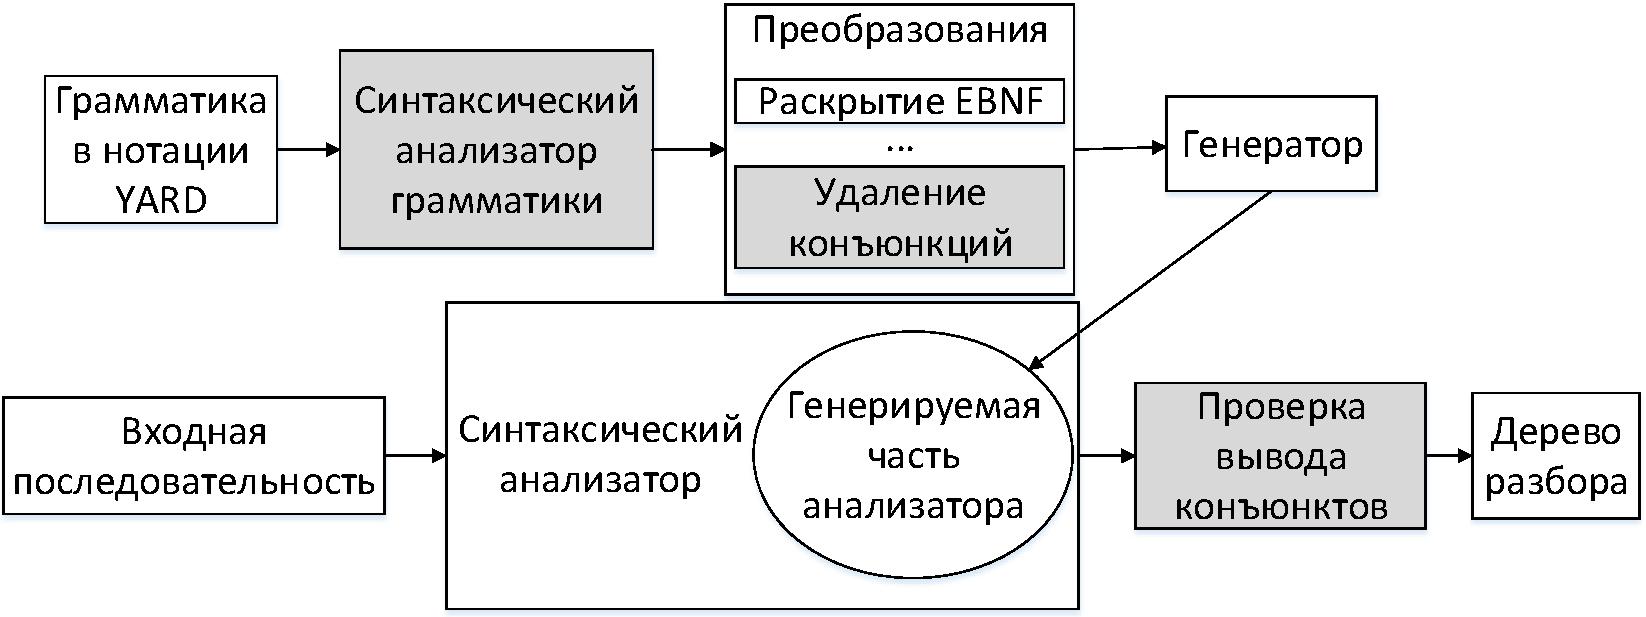
\includegraphics[width=\textwidth]{Gorokhov/courseworkpictures/img3.pdf}
\caption{Структура решения с учётом внесённых изменений}
\label{structure}
\end{figure}